% Options for packages loaded elsewhere
\PassOptionsToPackage{unicode}{hyperref}
\PassOptionsToPackage{hyphens}{url}
%
\documentclass[
  11pt,
  a4paper,
]{article}
\usepackage{amsmath,amssymb}
\usepackage{lmodern}
\usepackage{iftex}
\ifPDFTeX
  \usepackage[T1]{fontenc}
  \usepackage[utf8]{inputenc}
  \usepackage{textcomp} % provide euro and other symbols
\else % if luatex or xetex
  \ifXeTeX
    \usepackage{zxjatype} 
    \usepackage[ipaex]{zxjafont}
    \setromanfont{Times New Roman}
  \fi
  \usepackage{unicode-math}
  \defaultfontfeatures{Scale=MatchLowercase}
  \defaultfontfeatures[\rmfamily]{Ligatures=TeX,Scale=1}
\fi
% Use upquote if available, for straight quotes in verbatim environments
\IfFileExists{upquote.sty}{\usepackage{upquote}}{}
\IfFileExists{microtype.sty}{% use microtype if available
  \usepackage[]{microtype}
  \UseMicrotypeSet[protrusion]{basicmath} % disable protrusion for tt fonts
}{}
\usepackage{xcolor}
\IfFileExists{xurl.sty}{\usepackage{xurl}}{} % add URL line breaks if available
\IfFileExists{bookmark.sty}{\usepackage{bookmark}}{\usepackage{hyperref}}
\hypersetup{
  pdftitle={Text-Based Nudges Promoting Rubella Antibody Testing and Vaccination: Evidence from Nationwide Online Field Experiment in Japan},
  hidelinks,
  pdfcreator={LaTeX via pandoc}}
\urlstyle{same} % disable monospaced font for URLs
\usepackage[left=3cm,right=3cm,top=3cm,bottom=3cm]{geometry}

\usepackage{setspace}
\renewcommand{\baselinestretch}{1.5}
\usepackage{float}

\usepackage{longtable,booktabs,array}
\usepackage{threeparttable, threeparttablex, multirow}
\usepackage{calc} % for calculating minipage widths
% Correct order of tables after \paragraph or \subparagraph
\usepackage{etoolbox}
\makeatletter
\patchcmd\longtable{\par}{\if@noskipsec\mbox{}\fi\par}{}{}
\makeatother
% Allow footnotes in longtable head/foot
\IfFileExists{footnotehyper.sty}{\usepackage{footnotehyper}}{\usepackage{footnote}}
\makesavenoteenv{longtable}
\usepackage{graphicx}
\makeatletter
\def\maxwidth{\ifdim\Gin@nat@width>\linewidth\linewidth\else\Gin@nat@width\fi}
\def\maxheight{\ifdim\Gin@nat@height>\textheight\textheight\else\Gin@nat@height\fi}
\makeatother
% Scale images if necessary, so that they will not overflow the page
% margins by default, and it is still possible to overwrite the defaults
% using explicit options in \includegraphics[width, height, ...]{}
\setkeys{Gin}{width=\maxwidth,height=\maxheight,keepaspectratio}
% Set default figure placement to htbp
\makeatletter
\def\fps@figure{htbp}
\makeatother
\setlength{\emergencystretch}{3em} % prevent overfull lines
\providecommand{\tightlist}{%
  \setlength{\itemsep}{0pt}\setlength{\parskip}{0pt}}
\setcounter{secnumdepth}{5}


\usepackage{float}
\ifLuaTeX
  \usepackage{selnolig}  % disable illegal ligatures
\fi

\title{Text-Based Nudges Promoting Rubella Antibody Testing and Vaccination:
Evidence from Nationwide Online Field Experiment in Japan  \thanks{This study is conducted as a part of the Project ``Implementation of EBPM in Japan''
undertaken at the Research Institute of Economy, Trade and Industry (RIETI).
In completing this paper,
we thank participants of the EBPM Study Group and
the Discussion Paper Study Group of RIETI for their insightful comments.
This research is financially supported by
the Japan Society for the Promotion of Science
{[}JSPS Grant Number: 20H05632 (F., Ohtake){]}
and the Ministry of Health, Labor, and Welfare.
Prior to conducting a randomized controlled trial on an online survey,
this study was approved by the Institutional Review Board
of the Graduate School of Economics, Osaka University (R020114).}  }
\author{
    Hiroki Kato
  \thanks{Graduate School of Economics, Osaka University. E-mail: h-kato@econ.osaka-u.ac.jp  }
  \and
    Shusaku Sasaki
  \thanks{Center for Infectious Disease Education and Research, Osaka University.  }
  \and
    Fumio Ohtake
  \thanks{Graduate School of Economics, Osaka University.
Center for Infectious Disease Education and Research, Osaka University.  }
  \and
  }

\date{2022/04/15}



\begin{document}
\begin{spacing}{1}
  \maketitle
\end{spacing}
\begin{spacing}{1}
  \begin{abstract}
    This study conducted a randomized controlled trial (RCT) in a nationwide online survey
    to examine which text-based nudges best promote rubella antibody testing and vaccination.
    The main results are as follows.
    First, the altruistic message,
    which emphasizes that the fetus's health could be impaired by
    infecting women in the early stages of pregnancy with rubella,
    has a positive effect on the intention and behavior relating to the antibody test among men,
    who had automatically received a free coupon from the local government in 2019.
    Second, most people who test negative for antibodies (do not have antibodies),
    regardless of the type of nudge messages or whether or not they have received the coupon,
    have since been vaccinated.
    This result suggests that policies to increase antibody testing of pre-test individuals
    should be prioritized over those to increase vaccination of post-test negatives.
    Third, text-based messages have no statistically significant effect
    among men who had to apply for coupons themselves in 2019.
    
                \noindent
    \textbf{Key words}: Rubella, Vaccination, Antibody Test, Text-Based Nudges
        
        \noindent
    \textbf{JEL Codes}: D90, I12, I18
            
  \end{abstract}
\end{spacing}

\hypertarget{intro}{%
\section{はじめに}\label{intro}}

\hypertarget{background}{%
\section{日本における風しんワクチンの背景}\label{background}}

\hypertarget{experiment}{%
\section{オンライン調査の概要}\label{experiment}}

\hypertarget{result}{%
\section{Results}\label{result}}

\hypertarget{effect-of-text-based-nudges-on-intentions}{%
\subsection{Effect of Text-Based Nudges on Intentions}\label{effect-of-text-based-nudges-on-intentions}}

はじめに、我々は意向に対するナッジ・メッセージの効果を推定する。
ナッジ・メッセージによって行動変容を促したい対象は
第1回調査時点で抗体検査やワクチン接種を受けていない男性である。
そこで、第1回調査で過去に抗体検査とワクチン接種を受けていないと回答した人に限定したデータを用いる
(wave 1 selection data)。
さらに、我々の関心は
クーポン券の自動送付によってクーポン券を取得するための取引費用が減少したという意味での
インセンティブの有無のもとでのナッジ・メッセージの効果である。
そのために、2019年4月時点の年齢が46歳以下であるかどうかでサブサンプルを構築した。
自治体は2019年度に40歳から46歳の男性に無料クーポン券を送付し、
2020年度以降に47歳から56歳の男性にクーポン券を送付する。
二つのサブサンプルにおいて、個人の観察可能な特徴はトリートメント間でバランスされている。

また、検定力80\%・有意水準5\%を保つために必要な効果の規模を計算したところ、
2019年度にクーポン券が自動で送付される男性のサブサンプルを用いる場合、少なくとも
6.7
\%ポイントの差が必要である。
2019年度ではクーポン券を受け取るために手続きが必要な男性のサブサンプルを用いる場合、少なくとも
5
\%ポイントの差が必要である。

\begin{figure}[t]
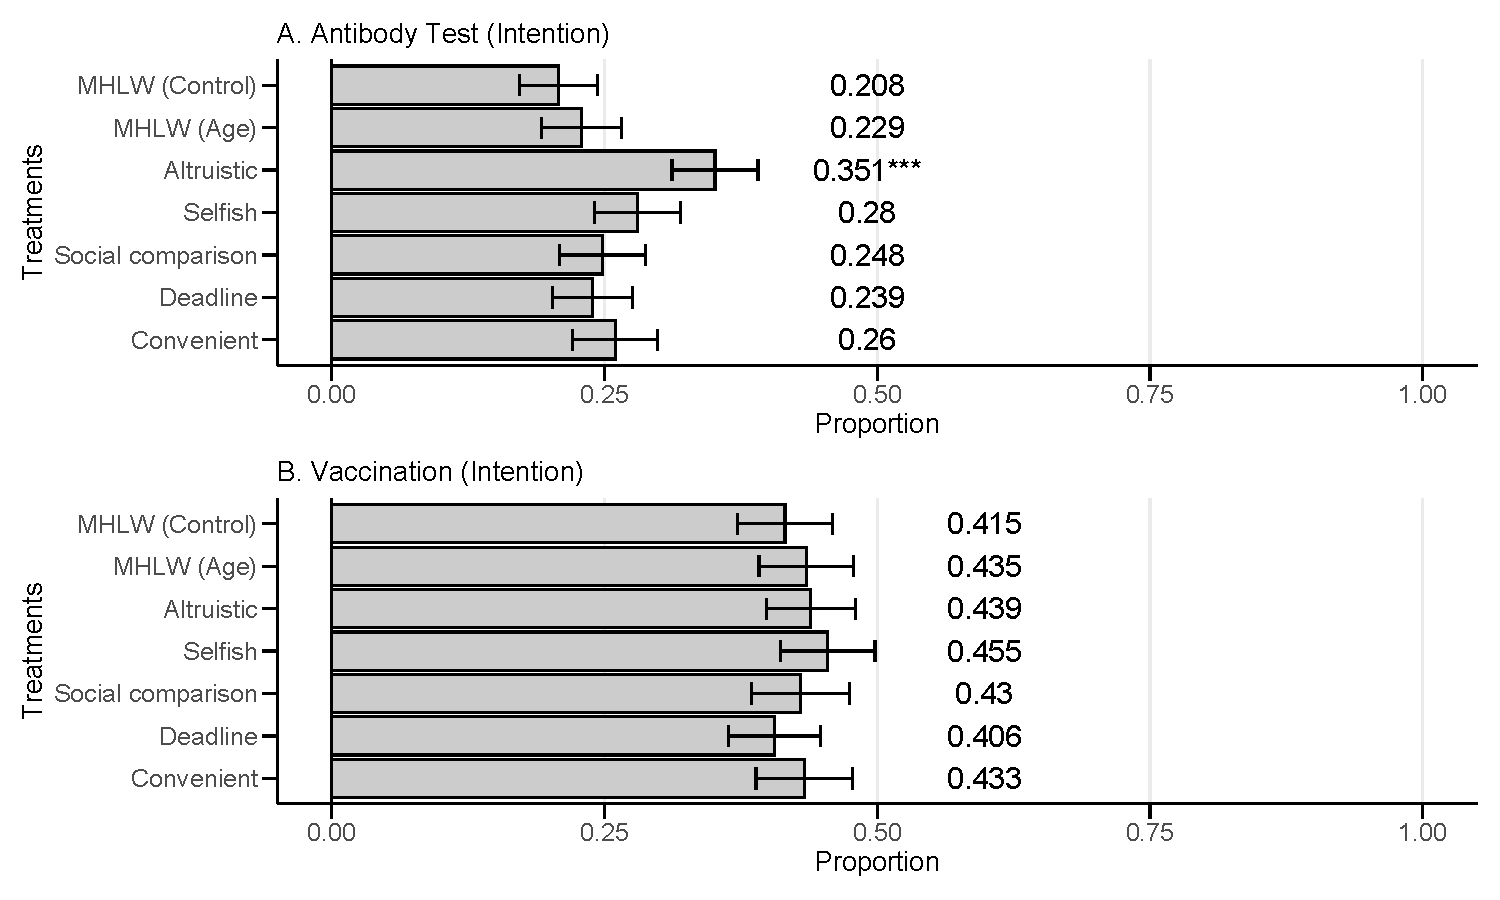
\includegraphics{C:/Users/katoo/Desktop/MHLW-Rubella-Project/2020-online-RCT/publish/body_files/figure-latex/int-coupon1-ttest-1} \caption{Effect of Text-Based Nudges on Intentions among Men for whom Coupons are Automatically Distributed in FY 2019. Data source: wave 1 selection data. Note: Numbers in the figure indicate the proportion of each group. Error bars indicate standard error of the mean. Asterisks are p-values for t-tests of the difference in means from the MHLW message group: * p < 0.1, ** p < 0.05, *** p < 0.01.}\label{fig:int-coupon1-ttest}
\end{figure}

2019年度にクーポン券が自動で送付される男性のサブサンプルを用いて、
我々は各介入群の抗体検査(パネルA)とワクチン接種(パネルB)の意向の比率を
図\ref{fig:int-coupon1-ttest}に示した。
その結果、利他強調メッセージは厚労省メッセージより抗体検査の意向を高めている。
厚労省メッセージ群の抗体検査の意向の比率は約20.8\%であるのに対して、
利他強調メッセージ群の抗体検査の意向の比率は約35.1\%である。
したがって、厚労省メッセージと比較して、
利他強調メッセージは抗体検査の意向を約14.3\%ポイント高めていて、
これは統計的に1\%水準で有意である。
また、厚労省メッセージと比較して、
すべてのナッジ・メッセージはワクチン接種の意向を統計的に有意に高めていない\footnote{また、すべての介入群のワクチン接種の意向の比率は抗体検査のそれよりも高い。
  これはワクチン接種の意向を引き出す質問の刺激によるものだと考えられる。
  我々はワクチン接種の意向を回答者に尋ねるとき、抗体を保有していないことを条件にしている。
  この条件がワクチン接種の必要性を強く刺激している可能性がある。}。

\begin{figure}[t]
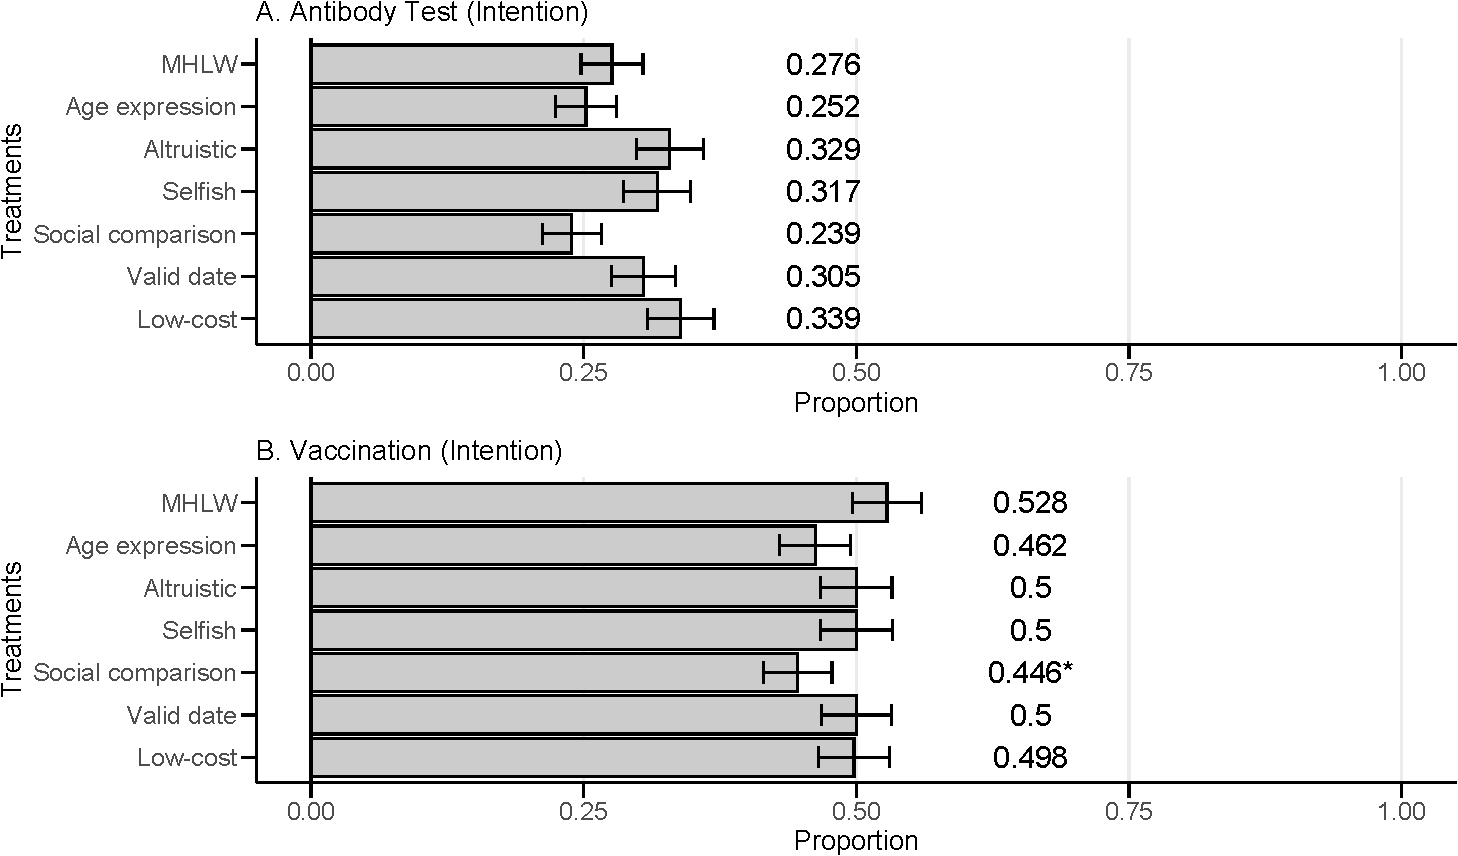
\includegraphics{C:/Users/katoo/Desktop/MHLW-Rubella-Project/2020-online-RCT/publish/body_files/figure-latex/int-coupon0-ttest-1} \caption{Effect of Text-Based Nudges on Intentions among Men Who Needed Costly Procedures to Receive Coupons in FY 2019. Data source: wave 1 selection data. Note: Numbers in the figure indicate the proportion of each group. Error bars indicate standard error of the mean. Asterisks are p-values for t-tests of the difference in means from the MHLW message group: * p < 0.1, ** p < 0.05, *** p < 0.01.}\label{fig:int-coupon0-ttest}
\end{figure}

2019年度にクーポン券を得るためにコストのかかる手続きが必要な男性のサブサンプルを用いて、
我々は各介入群の抗体検査(パネルA)とワクチン接種(パネルB)の意向の比率を
図\ref{fig:int-coupon0-ttest}に示した。
その結果、厚労省メッセージと比較して、
すべてのナッジ・メッセージは抗体検査の意向を統計的に有意に高めていない。
対照的に、
社会比較メッセージは厚労省メッセージよりもワクチン接種の意向を低めている。
厚労省メッセージのワクチン接種の意向比率は約52.8\%であるのに対し、
社会比較メッセージのワクチン接種の意向比率は約44.6\%である\footnote{2019年度にクーポン券が自動で送付される男性のサブサンプルを用いた結果と同様に、
  すべての介入群のワクチン接種の意向比率は抗体検査のそれよりも高い。
  これはワクチン接種の意向を引き出す質問の刺激によるものだと考えられる。}。
したがって、厚労省メッセージと比較して、
社会比較メッセージはワクチン接種の意向を約8.2\%ポイント低めており、
これは統計的に10\%水準で有意である。

この効果の原因の一つとして、ワクチン接種のただのりが挙げられる。
社会比較メッセージは「5人に1人が抗体を持っていない」ことを強調している。
裏返せば、5人に4人が抗体を持っているということである。
このメッセージを読んだ人は、
仮に風しんの抗体を保有していないとしても、全体の80\% が抗体を持っているので、
自身が感染する機会は少ないと考えたのかもしれない。
クーポン券を受け取るために手続きが必要なとき、
この信念がワクチンを接種することの価値を低め、
ワクチン接種の意向の比率を厚労省メッセージよりも下げた可能性がある。

クーポン券が自動的に送付されるかどうかは年齢で決まるので、
サブサンプルを用いたナッジ・メッセージの効果は
クーポン券が自動的に送付されるかどうかだけでなく、
二つのサブサンプルの年齢の違いの影響を受けている。
この問題を排除するために、意向の線形確率モデルを推定した。
説明変数はナッジ・メッセージのダミー変数、
ナッジ・メッセージのダミー変数とクーポン券が自動的に送付されることを示すダミー変数の交差項、
そして年齢を含んだ共変量である。
意向の線形確率モデルは上述の結果と同じ結果を得られた(詳細は補論を参照せよ)。

\hypertarget{effect-of-text-based-nudges-on-behaviors}{%
\subsection{Effect of Text-Based Nudges on Behaviors}\label{effect-of-text-based-nudges-on-behaviors}}

次に、我々は第1回調査以降の行動に対するナッジ・メッセージの効果を推定する。
第1回調査時点で抗体検査やワクチン接種を受けていない男性に焦点を当てるために、
第1回調査もしくは第2回調査で
第1回調査以前に抗体検査とワクチン接種を受けたと回答した人を排除した
(wave 2 selection data)\footnote{第1回調査以降に自身の接種歴を調べ直すなどによって、
  第1回調査と第2回調査の回答に違いが生じる可能性がある。
  そのため、
  どちらかの調査で第1回調査以前に抗体検査を受検したもしくはワクチンを接種したと回答した人を除いた。}。
さらに、
取引費用の減少の有無のもとでのナッジ・メッセージの効果を推定するために、
我々は2019年4月時点の年齢が46歳以下であるかどうかでサブサンプルを構築した。
二つのサブサンプルにおいて、個人の観察可能な特徴はトリートメント間でバランスされている。

また、検定力80\%・有意水準5\%を保つために必要な効果の規模を計算したところ、
2019年度にクーポン券が自動で送付される男性のサブサンプルを用いる場合、少なくとも
7.2
\%ポイントの差が必要である。
2019年度ではクーポン券を受け取るために手続きが必要な男性のサブサンプルを用いる場合、少なくとも
5.3
\%ポイントの差が必要である。

\begin{figure}[t]
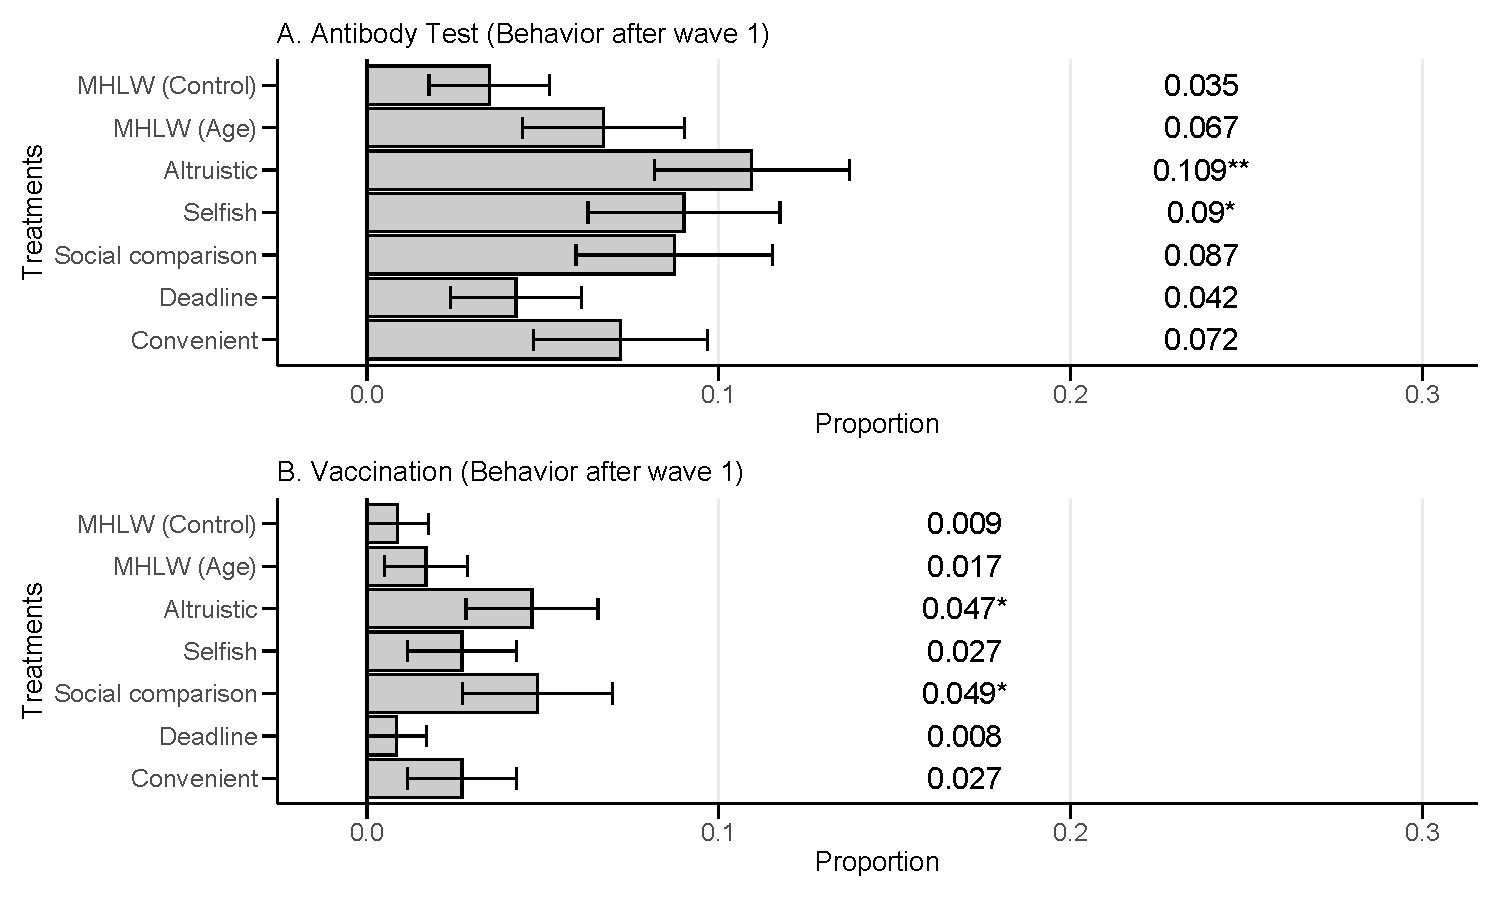
\includegraphics{C:/Users/katoo/Desktop/MHLW-Rubella-Project/2020-online-RCT/publish/body_files/figure-latex/act-coupon1-ttest-1} \caption{Effect of Text-Based Nudges on Behavior among Men for whom Coupons are Automatically Distributed in FY 2019. Data source: wave 2 selection data. Note: Numbers in the figure indicate the proportion of each group. Error bars indicate standard error of the mean. Asterisks are p-values for t-tests of the difference in means from the MHLW message group: * p < 0.1, ** p < 0.05, *** p < 0.01.}\label{fig:act-coupon1-ttest}
\end{figure}

2019年度にクーポン券が自動で送付される男性のサブサンプルを用いて、
我々は各介入群の抗体検査の受検率(パネルA)とワクチン接種率(パネルB)を
図\ref{fig:act-coupon1-ttest}に示した\footnote{ワクチン接種は抗体検査を受検し、
  ワクチンを接種したら1を取るダミー変数である。
  よって、ワクチン接種率はワクチン接種を通じて新規に抗体を獲得した人の比率とみなすこともできる。}。
その結果、利他強調メッセージと利己強調メッセージの抗体検査の受検率は厚労省メッセージよりも高い。
厚労省メッセージ群の抗体検査の受検率は約3.5\%である。
対して、利他強調メッセージ群と利己強調メッセージ群の抗体検査の受検率は
それぞれ約10.9\%と約9\%である。
したがって、厚労省メッセージと比較して、
利他強調メッセージは抗体検査の受検率を約7.4\%ポイント引き上げていて、
これは統計的に5\%水準で有意である。
また、利己強調メッセージは抗体検査の受検率を約5.5\%ポイント引き上げており、
これは統計的に10\%水準で有意である。

さらに、利他強調メッセージと社会比較メッセージのワクチン接種率は厚労省メッセージよりも高い。
厚労省メッセージ群のワクチン接種率は約0.9\%である。
対して、利他強調メッセージと社会比較メッセージのワクチン接種率は
それぞれ4.7\%と約4.9\%である。
したがって、厚労省メッセージと比較して、
利他強調メッセージと社会比較メッセージはワクチン接種率を
それぞれ約3.8\%ポイントと4\%ポイント引き上げていて、
これらは統計的に10\%水準で有意である。

\begin{figure}[t]
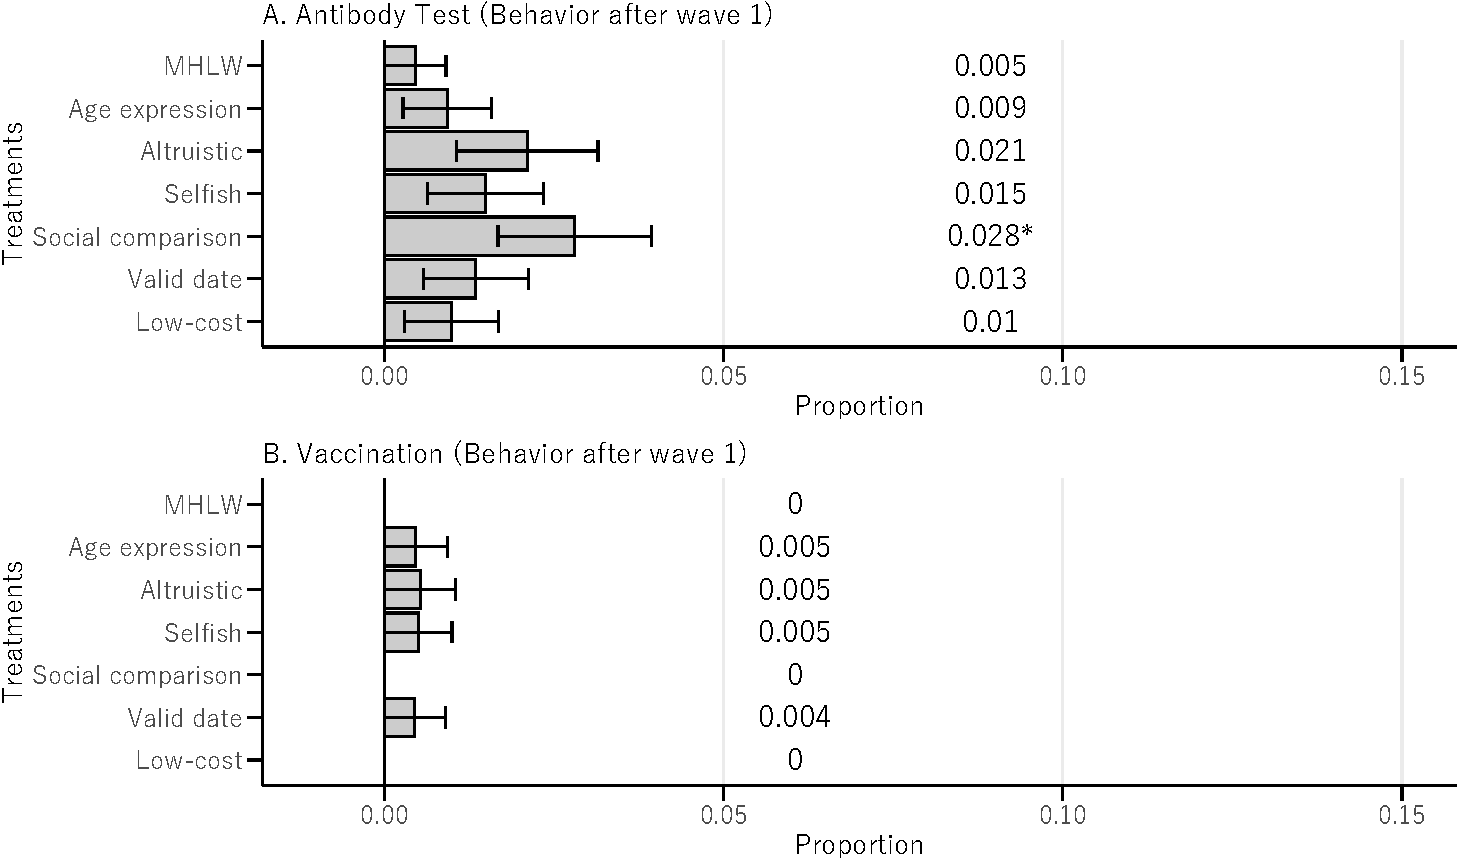
\includegraphics{C:/Users/katoo/Desktop/MHLW-Rubella-Project/2020-online-RCT/publish/body_files/figure-latex/act-coupon0-ttest-1} \caption{Effect of Text-Based Nudges on Behaviors among Men Who Needed Costly Procedures to Receive Coupons in FY 2019. Data source: wave 1 selection data. Note: Numbers in the figure indicate the proportion of each group. Error bars indicate standard error of the mean. Asterisks are p-values for t-tests of the difference in means from the MHLW message group: * p < 0.1, ** p < 0.05, *** p < 0.01.}\label{fig:act-coupon0-ttest}
\end{figure}

2019年度にクーポン券を得るためにコストのかかる手続きが必要な男性のサブサンプルを用いて、
我々は各介入群の抗体検査の受検率(パネルA)とワクチン接種率(パネルB)を
図\ref{fig:act-coupon0-ttest}に示した。
その結果、厚労省メッセージと比較して、
社会比較メッセージは抗体検査の受検率を高めているが、
ワクチン接種率を高めていない。
厚労省メッセージを読んだ人の0.5\%が抗体検査を受検しているが、
誰もワクチン接種をしていない。
同様に、社会比較メッセージを読んだ人の2.8\%が抗体検査を受検しているが、
誰もワクチン接種をしていない。
したがって、厚労省メッセージと比較して、
社会比較メッセージは抗体検査の受検率を約2.3\%ポイント引き上げていて、
これは統計的に10\%水準で有意である。
しかしながら、ワクチン接種率に対する効果はゼロである。

サブサンプルで推定されたナッジ・メッセージの効果は
クーポン券が自動的に送付されるかどうかだけでなく、
年齢の違いの影響を受けるので、
我々はこの問題を排除するために線形確率モデルを推定した。
行動の線形確率モデルは上述の結果と同じ結果を得られた。
それに加えて、2019年度にクーポン券が自動的に送付される男性において、
社会比較メッセージの抗体検査の受検率は厚労省メッセージよりも5.7\%ポイント高く、
これは統計的に10\%水準で有意である。

\hypertarget{conclusion}{%
\section{議論と結論}\label{conclusion}}

\newpage

\hypertarget{ux53c2ux8003ux6587ux732e}{%
\section*{参考文献}\label{ux53c2ux8003ux6587ux732e}}
\addcontentsline{toc}{section}{参考文献}

\end{document}
